%
% Capítulo 2
%
\chapter{Sistema de Gestão de Stocks} \label{cap2}

O sistema de gestão de stocks desenvolvido neste projeto, denominado Smart Stocks, é apresentado neste capítulo, bem como os requisitos funcionais e opcionais na secção \ref{subsec211}. Para uma melhor compreensão deste capítulo é recomendada a leitura do Anexo \ref{seca11}.

%
% Secção 2.1
%
\section{Sistema Smart Stocks} \label{sec21}
Smart Stocks é um sistema que visa dar suporte à gestão de stocks domésticos. Para tal é necessário recolher determinadas informações, tais como, as características da casa a gerir, as particularidades dos membros co-habitantes da casa e ainda os padrões de consumo e reposição. De forma a facilitar tal tarefa são disponibilizadas listas geridas pelo sistema. Por exemplo, lista de compras e lista dos itens em stock na casa, cuja consistência é garantida às custas dos movimentos de entrada e saída dos itens nos diversos locais de armazenamento.

%
% Subsecção 2.1.1
%
\subsection{Requisitos} \label{subsec211}
Como forma de assegurar as funcionalidades pretendidas para o sistema, são exigidos os seguintes requisitos funcionais e opcionais.

\paragraph{Requisitos Funcionais}
\begin{itemize}
	\item Informar o utilizador dos itens existentes, a sua validade e a sua quantidade;
	\item Alertar sobre os produtos que estão perto da data de validade;
	\item Gerar listas de compras com os produtos em falta;
	\item Possibilidade de especificar listas com os produtos a ter sempre em stock bem como as suas quantidades mínimas;
	\item Partilhar listas entre utilizadores da mesma casa;
	\item Criar de Listas;
	\item Especificação das alergias dos membros da casa.
\end{itemize}


\paragraph{Requisitos Opcionais}
\begin{itemize}
	\item Criar listas de produtos quase a expirar;
	\item Criar listas de produtos indesejados (Lista Negra);
	\item Criar listas de contenção em situações de emergência (Lista SOS);
	\item Inserir refeições extraordinárias de eventos a realizar num futuro próximo, para acrescentar alimentos não básicos à lista de compras.
\end{itemize}

%
% Subsecção 2.1.2
%
\subsection{Entidades} \label{subsec212}

Em seguida identificam-se as diversas entidades relevantes que compõem o sistema de informação, que permite gerir os itens em stock numa dada casa.
\subsubsection{Casa}
\begin{itemize}
	\item Cada casa é caracterizada por um identificador único, um nome, atribuído por um utilizador no momento de registo da casa. 
	\item Deve ser possível saber o número de bebés, crianças, adultos e seniores que vivem nessa casa.
	\item Uma casa está associada a um ou mais utilizadores, podendo um utilizador ter várias casas. 
	\item Podem existir um ou mais administradores de uma casa.
	\item A casa pode ter vários itens em stock.
	\item Para cada casa existem vários locais de armazenamento dos itens, por exemplo armários, frigoríficos, etc.
	\item Em cada casa deve ser possível conhecer as alergias assim como quantos membros possuem essa alergia (os membros não precisam necessariamente de estar registados).
\end{itemize}

\subsubsection{Utilizador}
\begin{itemize}
	\item Uma pessoa é representada por um utilizador que é caracterizado por um email ou por um nome de utilizador, pelo nome da pessoa, a sua idade e uma password.
\end{itemize}

\subsubsection{Listas}
\begin{itemize}
	\item Cada lista é composta por um identificador único e um nome.
	\item Uma lista pode ter vários produtos.
	\item Existem dois tipos de listas: de sistema e de utilizador. 
	\item As listas de sistema são comuns a todos os utilizadores registados, contudo são particulares a cada casa.	
	\item Um utilizador pode criar as suas listas, partilhando-as com outros utilizadores da casa ou tornando-as secretas.
\end{itemize}

\subsubsection{Categoria}
\begin{itemize}
	\item Uma categoria é identificada univocamente por um número ou por um nome.
\end{itemize}


\subsubsection{Produtos}
\begin{itemize}
	\item Um produto é constituído por um identificador único, um nome, se é ou não comestível, e a validade perecível.
	\item Para os produtos presentes numa lista pode ser possível saber a sua marca e a quantidade.
	\item Um produto pertence a uma categoria, podendo uma categoria ter vários produtos.
	\item Um produto pode ser concretizado por diversos itens em stock na casa.
\end{itemize}
 
\subsubsection{Item em Stock}
\begin{itemize}
	\item Um item em stock é a concretização de um produto que existe numa casa. É identificado univocamente por um número ou por uma marca, uma variedade e um segmento, é também caracterizado por uma descrição, o local de conservação, a quantidade e as datas de validade. 
	\item Para cada item deve ser possível saber os seus movimentos de entrada e saída de um local de armazenamento.
	\item Deve também ser possível saber os alergénios de cada item presente na casa.
\end{itemize}

\subsubsection{Movimento}
\begin{itemize}
	\item Para cada movimento deve ser possível saber o tipo do movimento (entrada ou saída), a data em que ocorreu e a quantidade de produtos. 
\end{itemize}

\subsubsection{Local de armazenamento}
\begin{itemize}
	\item Cada local de armazenamento é caraterizado por um identificador único, a temperatura e um nome.
	\item Deve ser possível saber a quantidade de cada item presente no local.
	\item Um local de armazenamento pode ter vários itens em stock presentes na casa e estar associado a diversos movimentos.
\end{itemize}

%
% Secção 2.2
%
\section{Arquitetura da Solução}\label{sec22}

Nesta secção pretende-se abordar de forma geral a solução implementada para resolver o problema apresentado na secção \ref{sec21}.

%
% Subsecção 2.2.1 Abordagem
%
\subsection{Abordagem}\label{subsec221}

\begin{figure}[H]
	\centering
	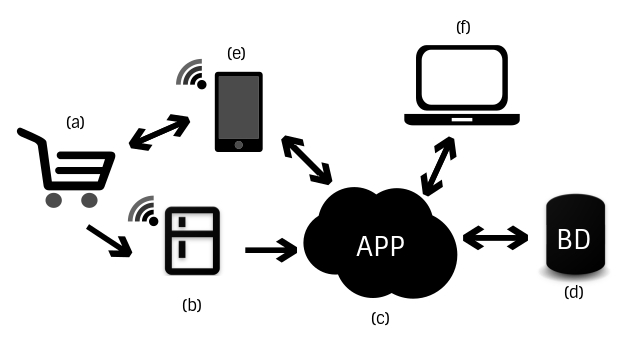
\includegraphics[width=16cm, height=8cm, scale=1]{./figures/architecture.png}
	\caption{Arquitetura Geral do Projeto}
	\label{project-general-architecture}
\end{figure}

Após uma ida às compras, os itens adquiridos, Figura \ref{project-general-architecture}(a), são armazenados nos seus respetivos locais, Figura \ref{project-general-architecture}(b). Como forma de automatizar a recolha de informação relativa quer aos artigos obtidos quer às suas caraterísticas, utilizam-se sensores. O uso destes só é possível caso os rótulos dos itens se encontrem em formato digital \textit{standard}, com \textit{tags} \acrfull{nfc} \cite{nfcforum:nfc} ou \acrfull{rfid} \cite{rfidinc:rfid}, e os locais de armazenamento contenham os respetivos leitores de \textit{tags}.

Ao guardar os artigos nos locais de armazenamento, os mesmos devem ser lidos pelos leitores, de forma a que a informação presente na \textit{tag} e o tipo de movimento (entrada ou saída) possam ser enviados para a API. Assim, estes dados são posteriormente tratados e armazenados de forma persistente na \acrfull{bd}, Figura \ref{project-general-architecture}(d). A APP, Figura \ref{project-general-architecture}(c), é responsável por retornar dados para as aplicações cliente, Figura \ref{project-general-architecture}(e, f). É ainda nesta que está presente o algoritmo de previsão de stocks utilizado para efetuar a previsão quanto à duração de cada um dos itens em stock.

No contexto da gestão de stocks assume-se a existência de duas formas de apresentação para os itens em stock: avulsos e embalados. Os primeiros são conservados em sistemas de arrumação identificados com \textit{tags} programáveis por \textit{smartphones}, \ref{project-general-architecture}(e). Os detalhes dos itens são especificados pelo utilizador e carregados para a \textit{tag}. Já os segundos contêm os seus rótulos digitais com o detalhe guardado pelos embaladores.\\

%
% Subsecção 2.2.2 Estrutura
%
\subsection{Arquitetura por Camadas}\label{subsec222}

O sistema de gestão de stocks é composto por 2 blocos principais: o bloco do lado do cliente e o bloco do lado do servidor, que se relacionam. A representação destes blocos é apresentada na Figura \ref{project-layers-structure}.

A arquitetura do projeto segue o padrão de arquitetura por camadas, dado que este padrão permite individualizar cada camada. Com isto, estas tornam-se independentes umas das outras, fornecendo não só abstração sobre as camadas inferiores, mas também, oferecendo a possibilidade de testar ou substituir cada uma das mesmas, sem que existam alterações significativas nas restantes.

\begin{figure}[H]
	\centering
	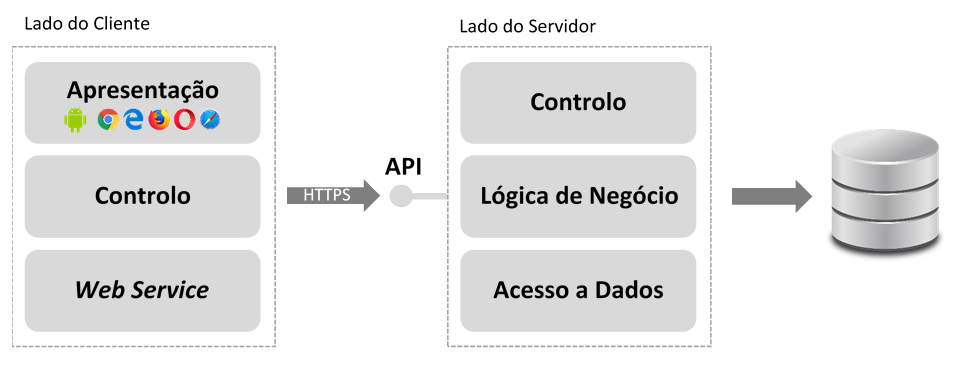
\includegraphics[width=\textwidth, scale=1]{./figures/project.png}
	\caption{Arquitetura por Camadas do Projeto}
	\label{project-layers-structure}
\end{figure}

No lado do cliente têm-se três camadas: a camada Apresentação que é responsável por representar os dados solicitados pelo utilizador; o Controlo que está encarregue de despoletar ações na camada do \textit{Web Service} de forma a satisfazer as solicitações do utilizador; e assim o \textit{Web Service} interage com a \gls{api-web}. 

As camadas que compõem o lado do servidor são: o Controlo que processa pedidos e retorna uma resposta; a camada da Lógica de Negócio que é responsável por satisfazer as regras de negócio; e por fim o Acesso a Dados que efetua leituras e escritas sobre a \acrshort{bd}.

\subsubsection{Tecnologias Inerentes à Solução}

O lado do servidor incluí três camadas e expõe uma \gls{api-web}. A \acrfull{dal} é produzida com a linguagem de programação \textit{Java}, usando a \acrfull{jpa}, e é responsável pelas leituras e escritas exercidas sobre a \acrfull{bd}. A \acrshort{bd} é externa ao servidor, utilizando para isso o \acrfull{sgbd} \textit{PostgreSQL}. A \acrfull{bll} é responsável pela aplicação das regras de negócio. A implementação desta camada é também realizada com linguagem \textit{Java}. Os \textit{controllers} foram desenvolvidos em \textit{Java} com a \textit{framework} da \textit{Spring}, chamada de \textit{Spring Boot}. A \gls{api-web} disponibiliza recursos em diferentes \textit{hypermedias}. Para a implementação do algoritmo de previsão de stocks usou-se a linguagem \textit{R}.

Do lado do cliente existem dois modos de interação, por uma aplicação móvel e outra por uma aplicação web. A aplicação móvel disponível para a plataforma \textit{Android}, desenvolvida em linguagem \textit{Kotlin}. A aplicação web é disponibilizada para a maioria dos browsers, e é implementada utilizando a linguagem \textit{JavaScript} no ambiente \textit{Node.js}, com o auxilio da \textit{framework Express}.